\section{Justification}
\paragraph{}
One of the major drawbacks of satellites is their poor temporal resolution. Although they can gather high quality data, they frequently lose contact with ground stations as they orbit. Therefore, their connection is limited to once every few hours. Astrea’s objective is to solve this issue by creating a network between ground stations and LEO satellites providing near real-time communication to the customer. A network like the aforementioned can only be carried out by a CubeSat constellation because they are economical and easily reproducible satellites, making their mass production affordable.

\paragraph{}
Another problem which is normally faced when designing a satellite is that the systems that contains become obsolete in a relatively short period of time. In order to prevent this premature obsolescence, we propose a constant refilling of the constellation, possible due to the low cost of CubeSat. Our preliminary study leads us to the fact that the orbit decay would make the CubeSats fall after 2 years of operation making us capable of updating the systems as the technology evolves.

\paragraph{}
Since 2013 CubeSat launches have experienced an incredible raise (as shown in Figure \ref{launches}) mainly because of their economic advantage. The future projection shows that the launches are going to continue increasing. However, more than the half of these CubeSat constellations are going to be focused on earth monitoring or become multiple-point sensors \cite{SpaceWorks}. In these situation, Astrea have the opportunity to take a unique position in the market, sharing the communication segment only with Kepler Communications\cite{keppler}.

\begin{figure}[H]
\centering
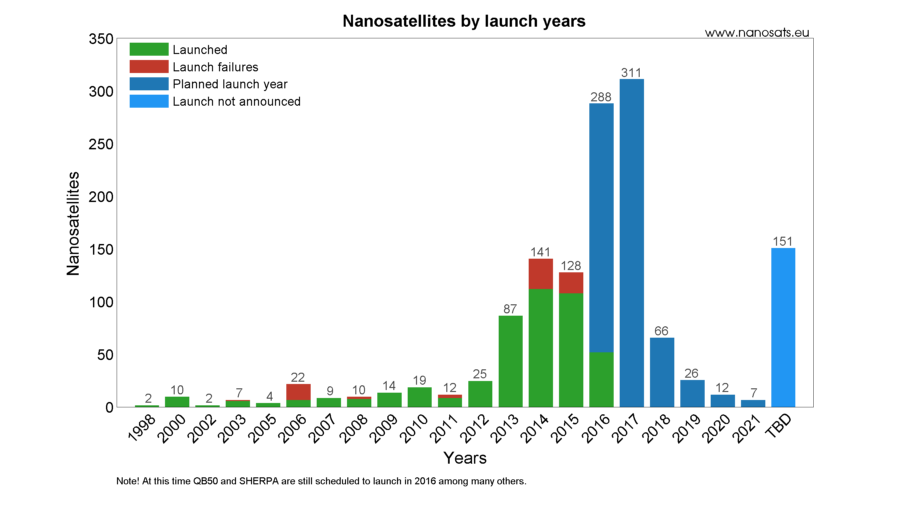
\includegraphics[scale=0.4]{img/launches.png}
\caption{Nanosatellites by launch years. Extracted from \cite{nanosats}}
\label{launches}
\end{figure}


\paragraph{}
Currently, there isn't any mission involving a large number of satellites implementing inter-satellite connection. However, missions like \textbf{QB-50} and \textbf{Keppler} are going to use this technology. The objective of these missions and other small satellites related projects is exposed at the Table 1
% \ref{currentsats}
. For Astrea, this is an intrinsic advantage since normally, the CubeSat that connects with ground won't necessary be the same that the one establishing a link with the customer satellite. This will enable client's satellites to configure and maintain dynamic routes and manage intermediate nodes.

%taula generada online. Sorry pel format estrany
\begin{table}[H]
\centering
\label{currentsats}
\begin{tabular}{|m{3.9cm}|m{3cm}|m{4cm}| m{4cm}|}
\hline
\begin{tabular}[c]{@{}c@{}}\textbf{Mission}\\ \textbf{Name}\end{tabular} & \begin{tabular}[c]{@{}c@{}}\textbf{Number of} \\ \textbf{satellites}\end{tabular} & \begin{tabular}[c]{@{}c@{}}\textbf{Launched/Projected}\\ \textbf{launch year}\end{tabular} & \multicolumn{1}{c|}{\begin{tabular}[c]{@{}c@{}}\textbf{Products or} \\ \textbf{Services}\end{tabular}} \\ \hline
\textit{Spire} & +100 & 2012 & Weather monitoring system. \\ \hline
\textit{GHSat} & 1 & 2013 & Greenhouse gas and air quality and gas emissions monitoring. \\ \hline
\textit{SpacePharma} & - & 2013 & Microgravity service with 3U CubeSats. \\ \hline
\textit{Sky and Space global} & 200 & 2015 & Communication service (voice,data and M2M) \\ \hline
\textit{Astro Digital} & 20 & 2015 & Earth Obervation\\& & &(Landmapper-HD). \\ \hline
\textit{EDSN} & 8 & 2015 & Demonstration of small satellite applications using consumer electronic-based nano-satellites. \\ \hline
\textit{QB-50} & 50 & 2016 & International network for thermo sphere exploration. \\ \hline
\textit{PROBA-3} & 2 & 2017 & Demonstrate the technologies needed for formation flying. \\ \hline
\textit{Keppler} & 50 & 2017 & Coordinate and relay the  communication between satellites and ground. \\ \hline
\end{tabular}
\caption{Current and future small satellites missions. Adapted from \cite{nanosats, ISC}}
\end{table}

